% Use only LaTeX2e, calling the article.cls class and 12-point type.

\documentclass[12pt]{article}

% Users of the {thebibliography} environment or BibTeX should use the
% scicite.sty package, downloadable from *Science* at
% www.sciencemag.org/about/authors/prep/TeX_help/ .
% This package should properly format in-text
% reference calls and reference-list numbers.

\usepackage{scicite}

% Use times if you have the font installed; otherwise, comment out the
% following line.

\usepackage{times}

% The preamble here sets up a lot of new/revised commands and
% environments.  It's annoying, but please do *not* try to strip these
% out into a separate .sty file (which could lead to the loss of some
% information when we convert the file to other formats).  Instead, keep
% them in the preamble of your main LaTeX source file.

\usepackage[usenames, dvipsnames]{color}
\usepackage{amsmath}
\usepackage[linesnumbered,boxed]{algorithm2e}
\usepackage{graphicx}
\usepackage{booktabs}
\usepackage{placeins}
% The following parameters seem to provide a reasonable page setup.

\topmargin 0.0cm
\oddsidemargin 0.2cm
\textwidth 16cm 
\textheight 21cm
\footskip 1.0cm



%The next command sets up an environment for the abstract to your paper.

\newenvironment{sciabstract}{%
\begin{quote} \bf}
{\end{quote}}


% If your reference list includes text notes as well as references,
% include the following line; otherwise, comment it out.

\renewcommand\refname{References and Notes}

% The following lines set up an environment for the last note in the
% reference list, which commonly includes acknowledgments of funding,
% help, etc.  It's intended for users of BibTeX or the {thebibliography}
% environment.  Users who are hand-coding their references at the end
% using a list environment such as {enumerate} can simply add another
% item at the end, and it will be numbered automatically.

\newcounter{lastnote}
\newenvironment{scilastnote}{%
\setcounter{lastnote}{\value{enumiv}}%
\addtocounter{lastnote}{+1}%
\begin{list}%
{\arabic{lastnote}.}
{\setlength{\leftmargin}{.22in}}
{\setlength{\labelsep}{.5em}}}
{\end{list}}


% Include your paper's title here

\title{PHY905 - Project 1} 


% Place the author information here.  Please hand-code the contact
% information and notecalls; do *not* use \footnote commands.  Let the
% author contact information appear immediately below the author names
% as shown.  We would also prefer that you don't change the type-size
% settings shown here.

\author
{Mengzhi Chen$^{1}$\\
\\
\normalsize{$^{1}$Department of Physics and Astronomy, NSCL/FRIB Laboratory}\\
\normalsize{Michigan State University, East Lansing, Michigan 48824, USA}\\
\\
\normalsize{$^\ast$To whom correspondence should be addressed; E-mail:  chenme24@msu.edu.}
}

% Include the date command, but leave its argument blank.

\date{Feburary 3, 2018}



%%%%%%%%%%%%%%%%% END OF PREAMBLE %%%%%%%%%%%%%%%%



\begin{document} 

% Set figure name

\renewcommand{\figurename}{Fig.}
\renewcommand{\tablename}{Tab.}
% partskip

\setlength{\parskip}{1ex}

% Double-space the manuscript.

\baselineskip18pt

% Make the title.

\maketitle 




% Place your abstract within the special {sciabstract} environment.

\begin{sciabstract}
  In this project, we implement three numerical solvers for one-dimensional Poisson's equation with Dirichlet boundary condition. The special solver has the highest efficiency but the narrowest application; the LU solver can be widely used but extremely slow. In addition, we show relative errors cannot decline all the way with the decreasing step size. 
\end{sciabstract}



% In setting up this template for *Science* papers, we've used both
% the \section* command and the \paragraph* command for topical
% divisions.  Which you use will of course depend on the type of paper
% you're writing.  Review Articles tend to have displayed headings, for
% which \section* is more appropriate; Research Articles, when they have
% formal topical divisions at all, tend to signal them with bold text
% that runs into the paragraph, for which \paragraph* is the right
% choice.  Either way, use the asterisk (*) modifier, as shown, to
% suppress numbering.
\section{Introduction}

Poisson's equation plays an important role in classical electrodynamics. It's a partial differential equation describing the potential field generated by given charge distributions. Under spherical symmetric situation, Poisson's equation has a form\cite{morten}
\[
\frac{1}{r^2}\frac{d}{dr}(r^2\frac{d\Phi}{dr}) = -4\pi\rho(r).
\]
With substitutions: $u(r) \to \Phi(r)r$, $-4\pi\rho(r)r \to f(r)$ and  $x \to r$. It becomes a one-dimensional second order differential equation written as
\[
-u''(x) = f(x).
\]
In this project, we solve this equation in the region $x \in(0,1)$ with the boundary conditions: $u(0) = u(1) =0$.
In order to solve equation numerically, we approximate $u(x)$ by n-1 discretized points and denote them as $v_i$ with $i = 1, 2, ... n$. The boundary conditions are: $v_0 = v_n = 0$, the spacing between two points is $h = 1/n$, so $v_i = v_0 + ih$. 
Taylor expanding $v_{i+1}$ and $v_{i-1}$ around $v_{1}$ gives
\begin{equation}
v_{i+1} = v_i + v'_ih + \frac{v''_i}{2}h^2 + \frac{v^{(3)}}{3!}h^3 + O(h^4), 
\end{equation}
\begin{equation}
v_{i-1} = v_i - v'_ih + \frac{v''_i}{2}h^2 - \frac{v^{(3)}}{3!}h^3 + O(h^4). 
\end{equation}
Add equation (1) and (2) and reorder terms, we get the three point formula
\begin{equation}
\frac{-(v_{i+1} + v_{i-1} - 2v_{i})}{h^2} = v''_i + O(h^2) \approx f_i,
\end{equation}
where $f_i = f(x_i)$. We can rewrite equation (3) as a group of linear equations with the form
\[
\mathbf{\hat{A}v = \bar{f}},
\]
where $\mathbf{v} = (v_1, v_2, ... v_n)^T$, $\mathbf{\bar{f}} = (f_1, f_2, ... f_n)^Th^2$ and $\mathbf{\hat{A}}$ is an $n \times n$ tridiagonal symmetric matrix of the form
\[   
\mathbf{\hat{A}} = \left[\begin{array}{cccccc}   
    2 &    -1    & 0   & \cdots  & \cdots  & 0\\   
    -1 &    2    & -1  & 0       & \cdots  & 0\\
    0 &    -1    & 2  & -1       & \cdots  & 0\\ 
    \vdots &    \vdots    & \ddots  & \ddots  & \ddots  & 0\\ 
    0 &    \cdots    & \cdots  & -1       & 2  & -1\\ 
    0 &    \cdots    & \cdots  & 0       & -1  & 2\\ 
\end{array}\right].   
\]
Our mission is then to develop solvers solving these equations.

In section 2, the general, special, LU decomposition solvers and their mathematical backgrounds are introduced. Three algorithms' complexities are listed. In section 3, solvers' performances are tested and their errors are analyzed. In the end, we summarize our work and draw conclusions in section 4.

\section{Method and algorithm}
\subsection{Gaussian elimination}
For a broader usage of our solver, suppose $\mathbf{\hat{A}}$ is a $n\times n$ general tridiagonal matrix, then equations take the form
\[   
\left[\begin{array}{cccccc}   
    b_1 &    c_1    & 0   & \cdots  & \cdots  & 0\\  
    a_1 &    b_2    & c_2  & 0       & \cdots  & 0\\
    0 &    a_2    & b_3  & c_3       & \cdots  & 0\\ 
    \vdots &    \vdots    & \ddots  & \ddots  & \ddots  & 0\\ 
    0 &    \cdots    & \cdots  & a_{n-2}       & b_{n-1}  & c_{n-1}\\ 
    0 &    \cdots    & \cdots  & 0       & a_{n-1}  & b_{n}\\ 
\end{array}\right]\left[\begin{array}{c}
     v_1\\    v_2\\ \cdots \\ \cdots\\ \cdots\\ v_{n}
 \end{array}\right] = \left[\begin{array}{c}
 \bar{f}_1 \\    \bar{f}_2   \\ \cdots\\ \cdots \\ \cdots \\ \bar{f}_n\\
 \end{array}\right]
\] 
We then do Gaussian elimination\cite{morten,sauer2012numerical} row by row. The first step is to subtract $\mathbf{\hat{A}_{21}}$ by following operation:
\[   
\left[\begin{array}{cccccc}   
    b_1 &    c_1    & 0   & \cdots  & \cdots  & 0 \\  
    a_1 &    b_2    & c_2  & 0       & \cdots  & 0\\
    0 &    a_2    & b_3  & c_3       & \cdots  & 0\\ 
    \vdots &    \vdots    & \ddots  & \ddots  & \ddots  & 0\\ 
    0 &    \cdots    & \cdots  & a_{n-2}       & b_{n-1}  & c_{n-1}\\ 
    0 &    \cdots    & \cdots  & 0       & a_{n-1}  & b_{n}\\ 
\end{array}\left|\begin{array}{c}
    \bar{f}_1 \\    \bar{f}_2   \\ \cdots\\ \cdots \\ \cdots \\ \bar{f}_n\\
 \end{array}\right]\right. \rightarrow \left[\begin{array}{cccccc}   
    b_1 &    c_1    & 0   & \cdots  & \cdots  & 0 \\  
    0 &    b_2 - \frac{a_1c_1}{b_1}    & c_2  & 0       & \cdots  & 0\\
    0 &    a_2    & b_3  & c_3       & \cdots  & 0\\ 
    \vdots &    \vdots    & \ddots  & \ddots  & \ddots  & 0\\ 
    0 &    \cdots    & \cdots  & a_{n-2}       & b_{n-1}  & c_{n-1}\\ 
    0 &    \cdots    & \cdots  & 0       & a_{n-1}  & b_{n}\\ 
\end{array}\left|\begin{array}{c}
    \bar{f}_1 \\  \bar{f}_2-\frac{c_1\bar{f}_1}{b}_1   \\ \cdots\\ \cdots \\ \cdots \\ \bar{f_n}\\
 \end{array}\right]\right.
 \] 
Repeat it until all $\mathbf{\hat{A}_{i+1,i}} (i = 1, 2 ... n-1)$ elements are eliminated. We can denote new diagonal elements as $\mathbf{\tilde{b}}$ and new $\mathbf{\bar{f}}$ as  $\mathbf{\tilde{f}}$. Formulas for them can be generalized
\begin{equation}
\tilde{b}_i = b_i - \frac{a_{i-1}c_{i-1}}{b_{i-1}}
\end{equation}
\begin{equation}
\tilde{f}_i = \bar{f}_i - \frac{\bar{f}_{i-1}c_{i-1}}{b_{i-1}}.
\end{equation}
Above substitutions start from $\tilde{b}_1 = b_1$ and $\tilde{f}_1 = \bar{f}_1$ in sequence of $i = 2, 3, ... n$. After these forward substitutions, the equations become
\[   
\left[\begin{array}{cccccc}   
    \tilde{b}_1 &    c_1    & 0   & \cdots  & \cdots  & 0\\  
    0 &    \tilde{b}_2    & c_2  & 0       & \cdots  & 0\\
    0 &    0   & \tilde{b}_3  & c_3       & \cdots  & 0\\ 
    \vdots &    \vdots    & \ddots  & \ddots  & \ddots  & 0\\ 
    0 &    \cdots    & \cdots  &0       & \tilde{b}_{n-1}  & c_{n-1}\\ 
    0 &    \cdots    & \cdots  & 0       & 0  & \tilde{b}_{n}\\ 
\end{array}\right]\left[\begin{array}{c}
     v_1\\    v_2\\ \cdots \\ \cdots\\ \cdots\\ v_{n}
 \end{array}\right] = \left[\begin{array}{c}
 \tilde{f}_1 \\    \tilde{f}_2   \\ \cdots\\ \cdots \\ \cdots \\ \tilde{f}_n\\
 \end{array}\right]
\] 
We then apply backward substitution from the last row. Starting from $v_n = \tilde{f}_n/\tilde{b}_n$, we can generalize expressions
\begin{equation}
u_i = \frac{\tilde{f}_i - c_{i}u_{i+1}}{\tilde{b}_i}
\end{equation}
where $i$ in sequence of $i = n-1, n-2, ... 1$. It stops until every $v_i$ is solved out. 

\subsection{A general solver}

As derived above, only non-zero elements of matrix matter in our calculation. Together with the fact that tridiagonal matrix is extremely sparse. It inspires us a great idea: instead of storing the whole matrix with a lot of useless zeros, why don't we only allocate space for three diagonal and off-diagonal vectors? By doing so, it saves us a lot of memory space and speeds up our algorithms by abandoning meaningless calculations. Based on these considerations, a general solver is implemented and the pseudocode is stated in Algorithm 1.
\begin{algorithm}
\caption{The general solver for tridiagonal matrix}
\KwIn{float vectors: $\vec{a}$, $\vec{b}$, $\vec{c}$ and $\vec{\bar{f}}$ from exact solution with length n+1}
\KwOut{solution: $\vec{u}$}
// Set Boundary conditions\;
$u_0 = u_{n} = 0$\;
// Forward Substitution\;
\For{$i=2;i \le n-2;i++$}
{
  $fac = c_i/b_i$\;
  $b_i = \bar{f}_i - (a_{i-1}*fac)$\;
  $\bar{f}_i = \bar{f}_i - (\bar{f}_{i-1}*fac)$\;
}
// Backward Substitution\;
$u_{n-1}=\bar{f}_{n-1}/b_{n-1}$\; 
\For{$i=n-2;i \ge 1;i--$}
{
  $u_i = (\tilde{f}_i - c_{i}u_{i+1})/b_i$\;
}
return $\vec{u}$\;
\end{algorithm}

We can see from above algorithm that by pre-calculating $c_i/b_i$, this general solver takes 8 FLOPS for one $u_i$. Thus, the total number of operations should be
\[
8(n-2) \sim \mathcal{O}(8n)\ \rm{FLOPS}.
\]


\subsection{A special solver}

As shown in section 2.1, for one dimensional Poisson's equation, the matrix $\mathbf{\hat{A}}$ is symmetric and all diagonal elements are 2 and off-diagonal elements equal to -1. By substituting these numbers into equation (4), we can generalize a simpler expression for $\tilde{b}_i$ as
\begin{equation}
\tilde{b}_i = \frac{i+1}{i} 
\end{equation}
Also, equation (5) and (6) can be simplify to forms
\begin{equation}
\tilde{f}_i = \bar{f}_i + \frac{\bar{f}_{i-1}}{b_{i-1}}.
\end{equation}
\begin{equation}
u_i = \frac{\tilde{f}_i + u_{i+1}}{\tilde{b}_i}
\end{equation}
Bases on above equations (7), (8) and (9), a special solver is then implemented and its pseudocode is stated in Algorithm 2.
\begin{algorithm}
\caption{The special solver for a special tridiagonal matrix}
\KwIn{float vectors: $\vec{b}$ and $\vec{\bar{f}}$ from exact solution with length n+1}
\KwOut{solution: $\vec{u}$}
// Set Boundary conditions\;
$u_0 = u_{n} = 0$\;
// Initialize $\vec{b}$\;
$b_i = (i + 1)/i$\;
// Forward Substitution\;
\For{$i=2;i \le n-2;i++$}
{
  $\bar{f}_i = \bar{f}_i + \bar{f}_{i-1}/b_{i-1}$\;
}
// Backward Substitution\;
$u_{n-1}=\bar{f}_{n-1}/b_{n-1}$\; 
\For{$i=n-2;i \ge 1;i--$}
{
  $u_i = (\tilde{f}_i +u_{i+1})/b_i$\;
}
return $\vec{u}$\;
\end{algorithm}
$\tilde{b_i}$ can be quickly calculated through vectorization. We can conclude from equations (8) and (9), that this special solver costs only 4 FLOPS for one $u_i$. Thus, the total number of operations should be
\[
4(n-2) \sim \mathcal{O}(4n)\ \rm{FLOPS}.
\]
Theoretically, the special solver speeds up a factor of 2 in certain problem compared with the general solver.

\subsection{LU decomposition and solver}
In linear algebra, it can be proved that an inevitable matrix $\mathbf{\hat{A}}$ can be LU(LU stands for lower and upper triangular matrices) decomposed. \cite{sauer2012numerical,golub2012matrix}. One intuitive way is through Gaussian elimination. LU decomposition in matrix form can be written as 
\[   
\mathbf{\hat{A}}=\mathbf{\hat{L}\hat{U}}=\left[\begin{array}{ccccc}   
    1 &    0    & 0   & \cdots    & 0\\  
    l_{21} &    1    & 0        & \cdots  & 0\\
    l_{31} &    l_{32}   &1        & \cdots  & 0\\ 
    \vdots      &\    & \cdots    & \ddots  & 0\\ 
    l_{n1} &     l_{n2}    &  l_{n3}  &\cdots   & 1\\ 
\end{array}\right]
\left[\begin{array}{ccccc}   
    u_{11} &    u_{12}    & u_{13}   & \cdots    & u_{1n}\\  
    0 &    u_{22}    &u_{23}        & \cdots  & u_{2n}\\
    0 &    0   &u_{33}        & \cdots  & u_{3n}\\ 
    \vdots      &\    & \cdots    & \ddots  & \vdots\\ 
    0 &     0    &  0  &\cdots   & u_{nn}\\ 
\end{array}\right].
\] 
So linear equations $\mathbf{\hat{A}v = \bar{f}}$ can be expressed as $\mathbf{\hat{L}(\hat{U}v) = \bar{f}}$. We then define an auxiliary vector $\mathbf{c}$ which satisfies $\mathbf{c = Uv}$. Then, we can divide problems into two steps.
\begin{itemize}
\item Step1: Solve $\mathbf{\hat{L}c = \bar{f}}$ for $\mathbf{c}$
\item Step2: Having c from last step, solve $\mathbf{\hat{U}u = c}$ to get $\mathbf{u}$
\end{itemize}

In the first step, L is a lower triangle matrix. So forward substitution is used in the first step. Starting from $c_1 = \bar{f}_1$, we get expressions for $c_i$
\begin{equation}
c_i = \bar{f}_i - \sum_{j=1}^{i-1}l_{ij}\bar{f}_j
\end{equation}
where $i = 2, 3, ...n-1$. We then use $\mathbf{c}$ to proceed the second step. In that step, backward substitution is used for U is an upper triangle matrix. (For clarification, when u has one subscript, it stands for elements from vector $\mathbf{u}$. Two subscripts mean element in matrix $\mathbf{\hat{U}}$). Starting from $u_{n-1} = c_{n-1}/u_{{n-1},{n-1}}$, we generalize formula for $u_i$
\begin{equation}
u_i = \frac{c_i - \sum_{j=i+1}^{n-1}u_{ij}u_j}{u_{ii}}
\end{equation}
where $i = n - 2, n - 3, ...1$. A solver bases on LU decomposition (LU solver) is implemented and shows in Algorithm 3\cite{sanderson2016armadillo}.

The complexity of LU decomposition is $\mathcal{O}(2/3n^3)$, same as general Gaussian decomposition. When we are solving $k$ linear equation sets with same $\mathbf{\hat{A}}$ but varying $\mathbf{\bar{f}}$, the total complexity of Gaussian elimination is $\mathcal{O}(2/3kn^3)$. At that time, LU decomposition shows superiority; because it only needs to deal with $\mathbf{\hat{A}}$ once and then does $k$ times substitutions. Its complexity is $\mathcal{O}(2/3n^3+kn^2)$ which has a large difference for large $n$ value.

\begin{algorithm}
\caption{LU decomposition solver}
\KwIn{float $(n-1)\times(n-1)$ matrix $\mathbf{\hat{A}}$ and $\vec{\bar{f}}$ from exact solution with length n+1}
\KwOut{solution: $\vec{u}$}
// Set Boundary conditions\;
$u_0 = u_{n} = 0$\;
// LU decomposition(using armadillo lib)\;
$lu(L, U, A)$\;
// Forward Substitution\;
\For{$i=2;i \le n-2;i++$}
{
    \For{$j=1;j \le i-1;j++$}
    {
     $c_i = \bar{f}_i + l_{ij}\bar{f}_j$\;
    }
}
$u_{n-1} = c_{n-1}/u_{n-1,n-1} $
// Backward Substitution\;
\For{$i=n-2;i \ge 1;i--$}
{
    \For{$j=i;j \le n-1;j++$}
    {
     $u_i = (c_i - u_{ij}u_j)$\;
    }
  $u_i = u_i/u_{ii}$
}
return $\vec{u}$\;
\end{algorithm}


\section{Problems, results and discussions}

\begin{itemize}
\item Clang compiler is used and codes are run on Macbook macOS High Sierra, 1.3 GHz Intel Core m7 processor. (see src repository for more information)
\item All data are average of three repetitions.
\end{itemize}

\subsection{Validity and efficiency}

We try to solve a system with $f(x)=100e^{-10x}$ and boundary conditions $u(x=0)=u(x=1)=0$. It has an analytic solution $u(x)=1-(1-e^{-10})x-e^{-10x}$ for verification.

The general solver is tested with different steps by setting $n = 10, 100$ and 1000. The analytic and numerical results are shown in figure 1. We can see that when $n = 10$, the numerical error is quite large. However, as $n$ increases to 100 and 1000, we can hardly see differences between analytic and numerical solutions. For further analysis of errors, we need a more quantitative discussion.

\begin{figure}[h!]
\centering
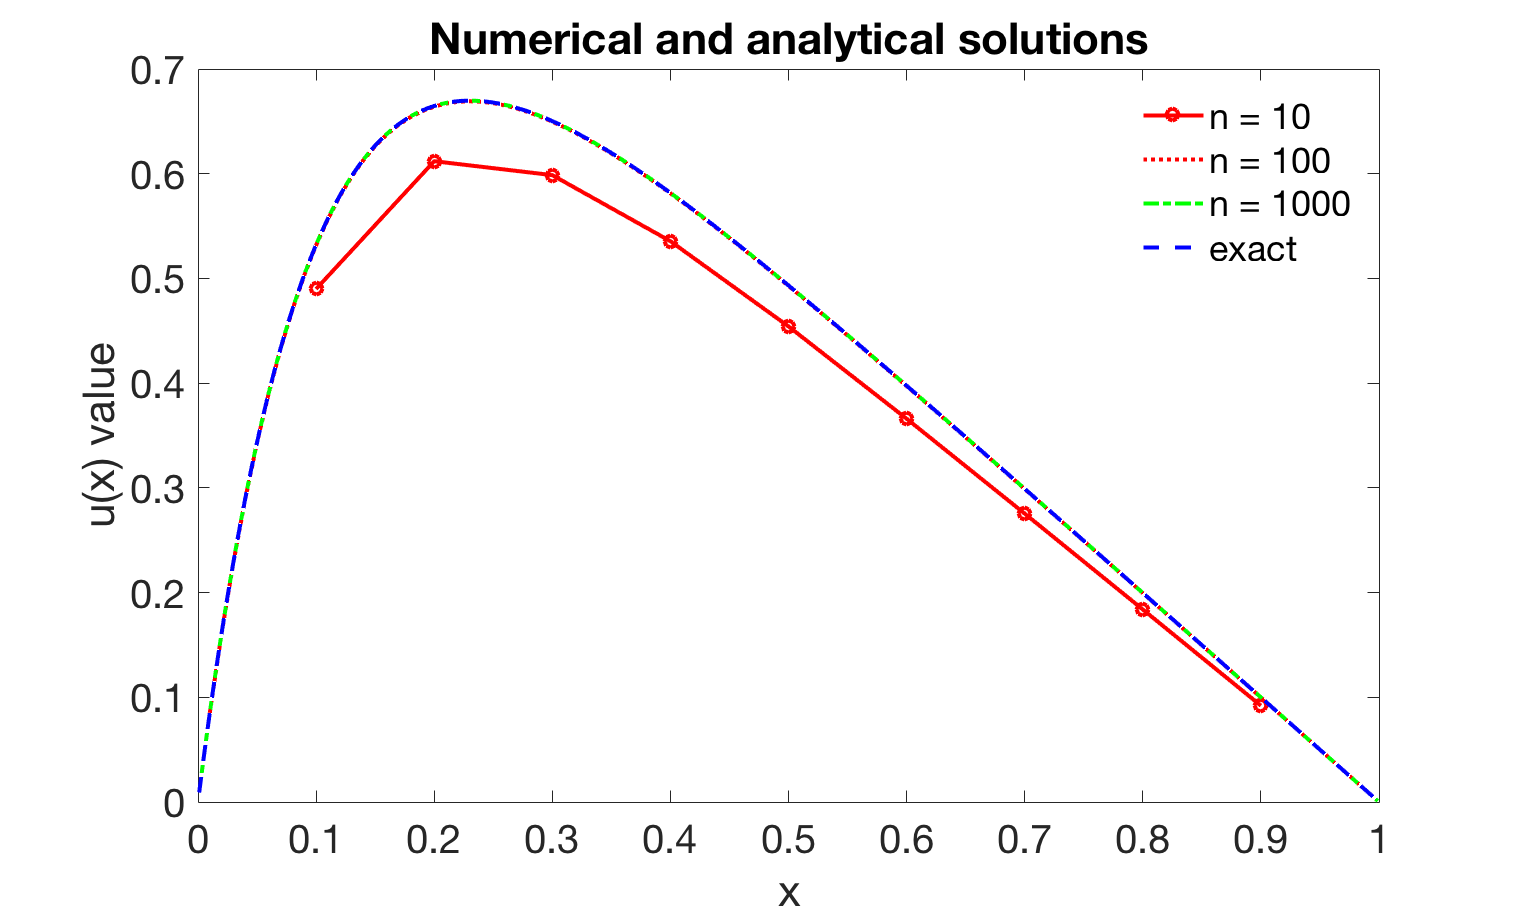
\includegraphics[width=14cm,height=8cm]{c.png}
\caption{Analytic and numerical solutions for n = 10, 100 and 1000 in interval (0,1).}
\label{fig:1}
\end{figure}

As we discussed in section 2.2, the special solver has a higher efficiency in this problem. Therefore, we would like to verify this point. In table 1, execution times for two solvers with increasing $n$ up to $10^7$ are listed (only forward and backward substitution processes are included). As we can see, the special solver does have higher efficiency. However, it can't reduce half of the execution as predicted. We believe it's normal because we only cut down half of FLOPS. There are still overheads coming from loop initialization, data reading and writing, etc where we do nothing on. Luckily, as increasing $n$, programs become more compute bound which means we can save more time by using special solver.

\begin{table}[]
\centering
\begin{tabular}{ccc}
\toprule
Size n & \multicolumn{1}{l}{\begin{tabular}[c]{@{}l@{}}Execution time of \\ General Solver (ms)\end{tabular}} & \multicolumn{1}{l}{\begin{tabular}[c]{@{}l@{}}Execution time of \\ Special Solver (ms)\end{tabular}} \\
\midrule
$10^1$ & 0.003 & 0.003 \\
$10^2$ & 0.005 & 0.004 \\
$10^3$ & 0.042 & 0.019 \\
$10^4$ & 0.330 & 0.227 \\
$10^5$ & 2.850 & 2.380 \\
$10^6$ & 25.876 & 23.508 \\
$10^7$ & 253.118 & 197.520\\
\bottomrule
\end{tabular}
\caption{Execution times for general and special solvers for several different size $n$.}
\label{my-label}
\end{table}

\subsection{Error analysis}
Driven by the motivation of increasing numerical precision, we carry out an error analysis for our solvers.

As stated in reference\cite{morten2}, the total error comes from both truncation approximation and round-off error. It can be written as
\[
\epsilon_{tot} = \epsilon_{app}+\epsilon_{ro}.
\]
In our case of using three point formula and one FLOP for double precision numbers, 
\[
\epsilon_{app} \approx \frac{f_{0}^{(4)}}{12}h^2;\ \ \ 
\left|\epsilon_{M}\right| \le 10^{-15};
\]
\begin{equation}
\left|\epsilon_{tot}\right| \le \frac{f_{0}^{(4)}}{12}h^2 + \frac{2\epsilon_M}{h^2}.
\end{equation}
In order to get suitable $h$, we calculate the derivative of $\left|\epsilon_{tot}\right|$ with regard to $h$ in equation (12). When
\begin{equation}
h = (\frac{24\epsilon_M}{f_{0}^{(4)}})^{1/4},
\end{equation}
it gives the minimum total error. Using formula $f(x=1)$ in our problem, we get $h\sim10^{-5}$. In order to see how total error varies with spacing $h$ ($h=1/n$), we define logarithm relative error as 
\[
\epsilon_i = \log_{10}\left(\left|\frac{u_i-u_i(exact)}{u_i(exact)}\right|\right).
\]
In figure 2, we show how $max(\epsilon_i)$ varies with $\log_{10}h$. At the same time, some of these values are listed in table 2. We can see both solvers have the lowest error at about $h\sim10^{-5}-10^{-6}$. It agrees with our previous prediction. In the large $h$ region, truncation error dominates, so we can see two solvers have identical errors because they use the same formula. After the lowest point, relative error grows with decreasing $h$ because round-off error dominates now; it also explains why two solvers behave diversely at small $h$ region. Their different calculation processes bring distinct round-off errors.  

In a word, we can not achieve infinite small error; so we should better set the step size to gain high efficiency and accuracy.
\begin{figure}[h!]
\centering
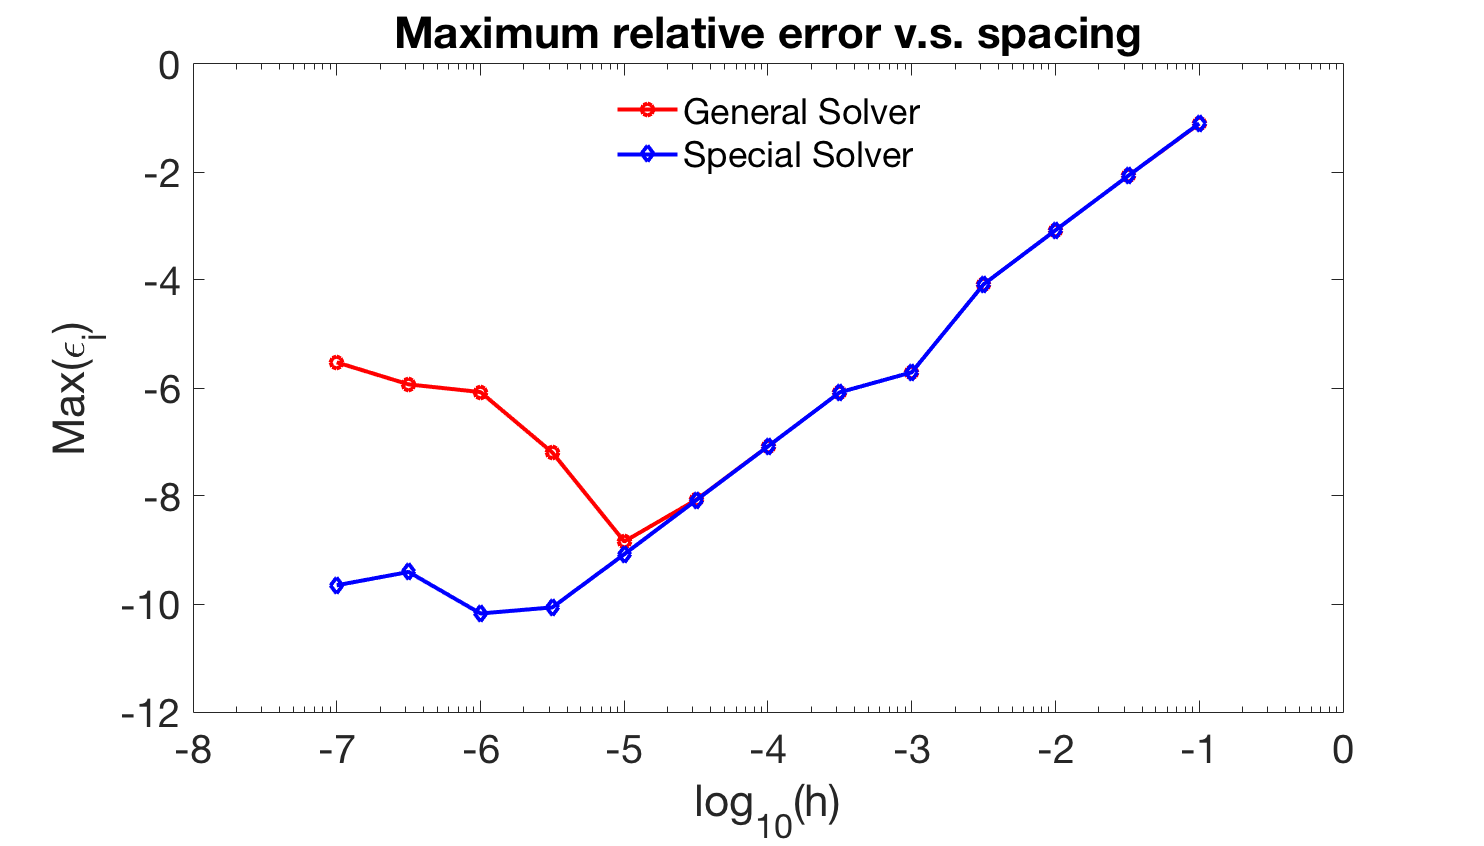
\includegraphics[width=14cm,height=8cm]{e.png}
\caption{Maximum logarithm relative errors for general and special solvers with different spacing}
\label{fig:2}
\end{figure}

\begin{table}[]
\centering
\begin{tabular}{cccc}
\toprule
Size n & Spacing h &\multicolumn{1}{l}{\begin{tabular}[c]{@{}l@{}}Maximum $\epsilon_i$ of \\ General Solver \end{tabular}} & \multicolumn{1}{l}{\begin{tabular}[c]{@{}l@{}}Maximum $\epsilon_i$ of \\ Special Solver \end{tabular}} \\
\midrule
$10^1$ & $10^{-1}$  & -1.1006  & -1.1006  \\
$10^2$ & $10^{-2}$ &-3.0794  & -3.0794   \\
$10^3$ & $10^{-3}$ &-5.7092   & -5.7092 \\
$10^4$ & $10^{-4}$ &-7.0792  & -7.0792 \\
$10^5$ & $10^{-5}$ &-8.8430  & -9.0790   \\
$10^6$ & $10^{-6}$ &-6.0755 & -10.1757\\
$10^7$ & $10^{-7}$ &-5.5252 & -9.6534\\
\bottomrule
\end{tabular}
\caption{Relative errors for general and special solvers for several different size $n$.}
\label{my-label}
\end{table}

\FloatBarrier
\subsection{Comparison with LU solver}
To show the superiority of our solvers, I compared the execution times of general, special and LU solvers. The results are shown in table 3. As we can see, the execution time of LU solver increases extremely fast compared with others. It can be explained as we stated in section 2. The complexity of LU solver is $\mathcal{O}(2/3n^3)$ and others two are $\mathcal{O}(kn)$.

There is also one more thing worth noticing. We are not able to attain results for $n>10^5$. A $10^6 \times 10^6$ double precision matrix occupies more than 900 GB space; nevertheless, there is not enough space to store it in a personal computer. Eventually, it leads a collapse of LU solver. 

The Special solver is faster than the general one; they two are much faster than the LU solver. But we should keep in mind that the LU solver can be applied to any linear equations and the general solver can deal with general tridiagonal matrix; but special solver only works with our problem. In sum, the moment we get efficiency is also the minute we lose generality. Sometimes, we have to trade off carefully between these two.

\begin{table}[]
\centering
\begin{tabular}{cccc}
\toprule
Size n   & \begin{tabular}[c]{@{}l@{}}Execution time of\\ General Solver (ms)\end{tabular} & \begin{tabular}[c]{@{}l@{}}Execution time of \\ Special Solver (ms)\end{tabular} & \begin{tabular}[c]{@{}l@{}}Execution time of \\ LU decomposit Solver (ms)\end{tabular} \\
\midrule
$10^1$ & 0.003    & 0.003   & 0.045    \\
$10^2$ & 0.005   & 0.004    & 0.748  \\
$10^3$  & 0.042  & 0.019  & 75.208    \\
$10^4$   & 0.330  & 0.227  & 46590.267  \\
$10^5$   & 2.850  & 2.380  & Nan  \\
$10^6$  & 25.876  & 23.508  & Nan   \\
$10^7$ & 253.118  & 197.520 & Nan \\                  
\bottomrule
\end{tabular}
\caption{Execution times for general, special and LU solvers for several different size $n$.}
\label{my-label}
\end{table}

\section{Summary and conclusions}
In this project, we develop the general and special solvers for numerically solving one-dimensional Poisson's equation. Their correctness is verified by solving $f(x)=100\exp^{-10x}$ whose analytically solution is known. Through measurement of their execution times, we see that the special solver has higher efficiency but the general solver can be broadly used to any tridiagonal matrix. Error analysis indicates only the appropriate $n$ gives the smallest total relative error. It inspires us to carefully choose step size to get both high efficiency and precision. In our case, $n = 10^6$ is the best choice for the special solver.

In addition, these two solvers are compared with the LU solver. The general and special solvers show superior speed advantage. However, they also have a narrower range of application (tridiagonal matrix only). On the contrary, the LU solver can deal with any matrix but may subject to limited memory space and low speed. We should carefully choose solvers for specific problems. As we are solving a one-dimensional Poisson's equation, the special solver should be our top option。

\section{Comments}
Personally speaking, I think this project is very suitable as a beginning of our course. It combines widely seen Poisson's equation with basic linear equations solvers. Professor also reminds us some important points in the numerical calculation such as the origin of errors, algorithms selecting. I appreciate patience guidance from Professor Morten. I also look forward to learning more from future projects.



% Your references go at the end of the main text, and before the
% figures.  For this document we've used BibTeX, the .bib file
% scibib.bib, and the .bst file Science.bst.  The package scicite.sty
% was included to format the reference numbers according to *Science*
% style.


\bibliography{scibib}

\bibliographystyle{Science}

\end{document}




















